% !TeX root = RJwrapper.tex
\title{Current status and propsects of R-packages for the design of
experiments}
\author{by Emi Tanaka}

\maketitle

\abstract{%
The critical role of data collection is well captured in the expression
``garbage in, garbage out'\,' -- in other words, if the collected data
is rubbish then no analysis, however complex it may be, can make
something out of it. The gold standard for data collection is through
well-designed experiments. Re-running an experiment is generally
expensive and in some cases difficult due to limited resources, The
design of experiment is important in getting a good value out of the
collected data. In this article I describe the current state of the
R-packages for the design of experiments through textual analysis and
download trends. I discuss also the software design of widely utilised R
packages in the field and conclude with discussion of some future
prospects for the field.
}

\hypertarget{introduction}{%
\section{Introduction}\label{introduction}}

\hypertarget{explorative-analysis}{%
\section{Explorative Analysis}\label{explorative-analysis}}

\hypertarget{what-are-the-common-types-of-experimental-designs}{%
\subsection{What are the common types of experimental
designs?}\label{what-are-the-common-types-of-experimental-designs}}

\hypertarget{how-do-packages-interplay-with-each-other}{%
\subsection{How do packages interplay with each
other?}\label{how-do-packages-interplay-with-each-other}}

\hypertarget{which-packages-are-widely-utilised}{%
\subsection{Which packages are widely
utilised?}\label{which-packages-are-widely-utilised}}

\hypertarget{software-design}{%
\section{Software Design}\label{software-design}}

\hypertarget{propsects-and-discussion}{%
\section{Propsects and Discussion}\label{propsects-and-discussion}}

\newpage

\begin{Schunk}
\begin{table}

\caption{\label{tab:bigram-title}The bigram of the R-package titles as provided in the DESCRIPTION file in CRAN.}
\centering
\begin{tabular}[t]{lr}
\toprule
Bigram & Count\\
\midrule
optimal design & 10\\
experimental design & 8\\
clinical trial & 5\\
dose finding & 5\\
sequential design & 5\\
block design & 4\\
microarray experiment & 4\\
response surface & 4\\
\bottomrule
\end{tabular}
\end{table}

\end{Schunk}

\begin{Schunk}
\begin{table}

\caption{\label{tab:bigram-desc}The bigram of the R-package descriptions as provided in the DESCRIPTION file in CRAN.}
\centering
\begin{tabular}[t]{lr}
\toprule
Bigram & Count\\
\midrule
experimental design & 11\\
optimal design & 10\\
package provide & 7\\
response surface & 7\\
factorial design & 6\\
graphical user & 6\\
user interface & 6\\
block design & 5\\
contour plot & 5\\
design based & 5\\
effect model & 5\\
fractional factorial & 5\\
microarray experiment & 5\\
mixed effect & 5\\
provide function & 5\\
sample size & 5\\
sequential design & 5\\
\bottomrule
\end{tabular}
\end{table}

\end{Schunk}

\begin{Schunk}


\begin{center}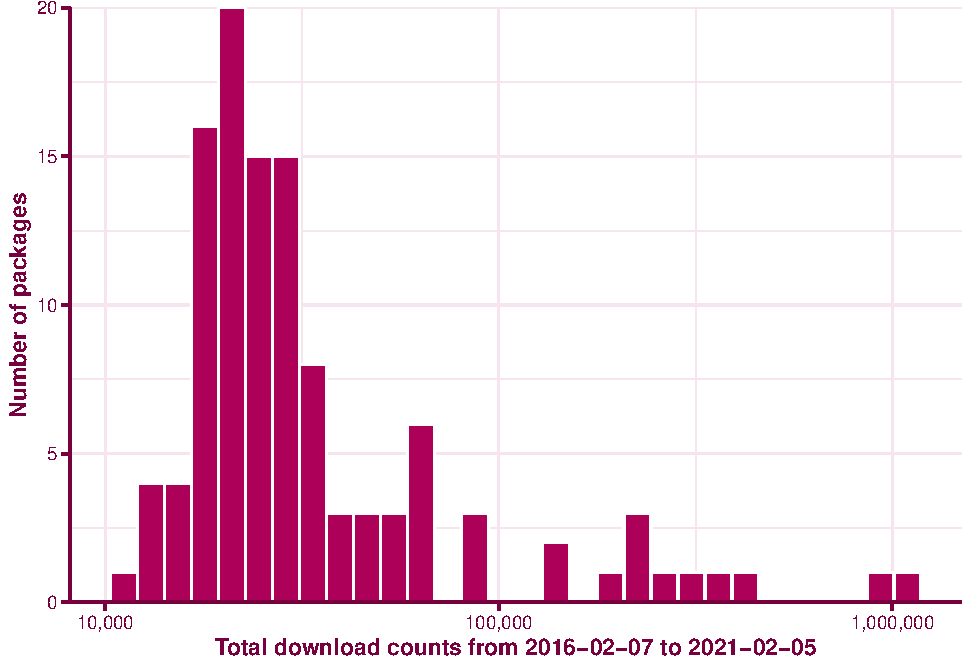
\includegraphics{paper_files/figure-latex/download-hist-1} \end{center}

\end{Schunk}

\begin{Schunk}
\begin{Soutput}
#>  [1] "agricolae"   "AlgDesign"   "conf.design" "DiceDesign"  "DiceKriging"
#>  [6] "DoE.base"    "ez"          "FrF2"        "lhs"         "rsm"
\end{Soutput}
\end{Schunk}

\begin{Schunk}


\begin{center}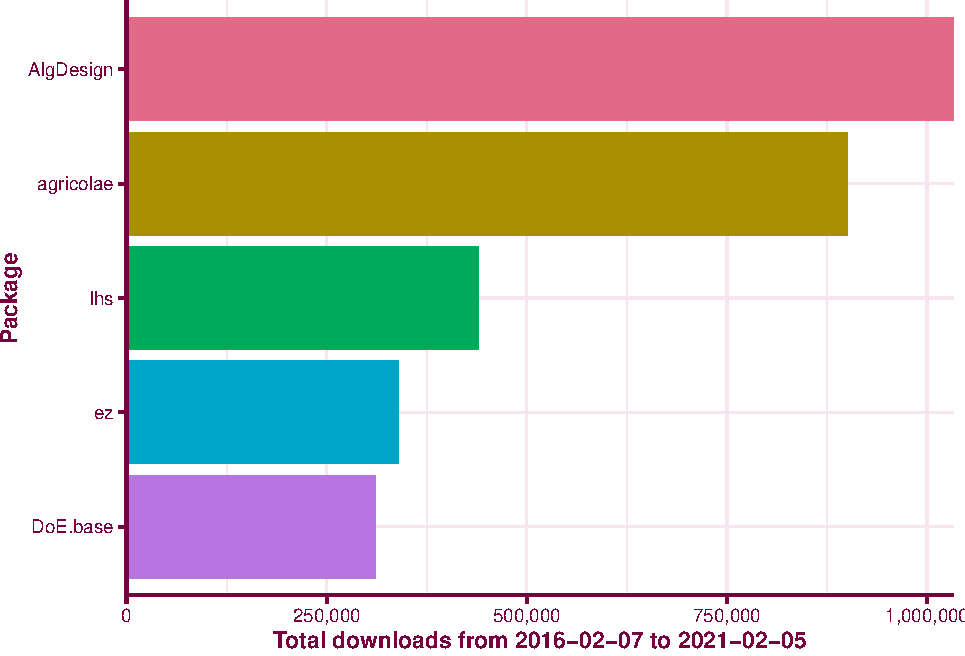
\includegraphics{paper_files/figure-latex/download-barplot-1} \end{center}

\end{Schunk}

\begin{Schunk}


\begin{center}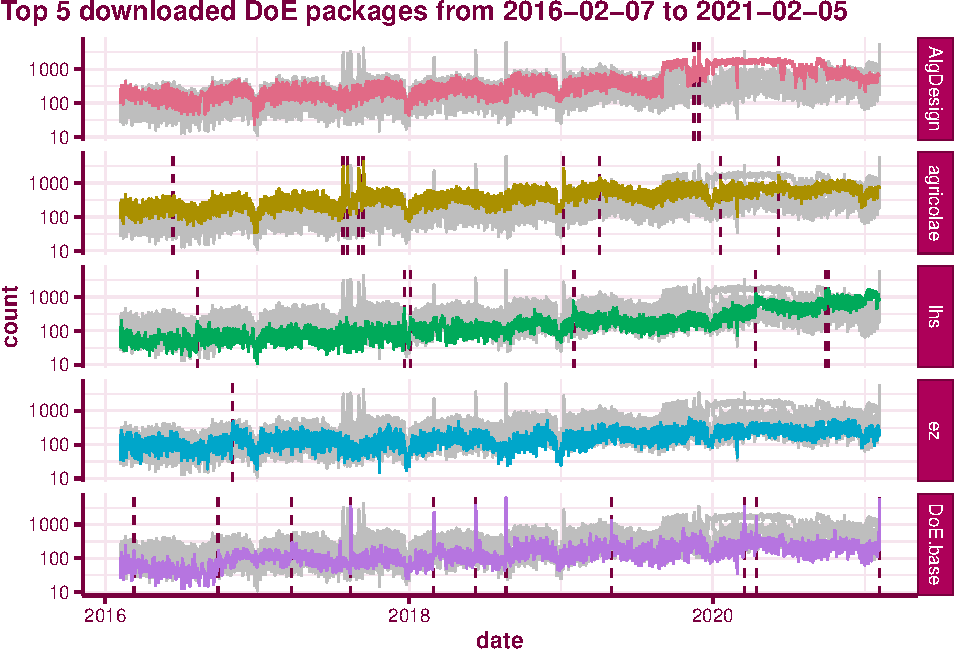
\includegraphics{paper_files/figure-latex/download-timeplot-1} \end{center}

\end{Schunk}

\hypertarget{introduction-1}{%
\subsection{Introduction}\label{introduction-1}}

\texttt{test} \code{test}

\CRANpkg{agricolae}

\ctv{ExperimentalDesign}

\ctv{OfficialStatistics}

\hypertarget{helping-info-to-get-started}{%
\subsection{Helping info to get
started}\label{helping-info-to-get-started}}

Introductory section which may include references in parentheses
\citep{R}, or cite a reference such as \citet{R} in the text.

\hypertarget{section-title-in-sentence-case}{%
\subsection{Section title in sentence
case}\label{section-title-in-sentence-case}}

Let's check fi this works Figure @ref(fig:Rlogo).

This section may contain a figure such as Figure \ref{fig:Rlogo}.

\begin{Schunk}
\begin{figure}[htbp]

{\centering 
\includegraphics[width=2in]{/Users/etan0038/Dropbox/projects/paper-review-DoE-pkgs/Rlogo} 

}

\caption[The logo of R]{The logo of R.}\label{fig:Rlogo}
\end{figure}
\end{Schunk}

\hypertarget{summary}{%
\subsection{Summary}\label{summary}}

This file is only a basic article template. For full details of
\emph{The R Journal} style and information on how to prepare your
article for submission, see the
\href{https://journal.r-project.org/share/author-guide.pdf}{Instructions
for Authors}.

\hypertarget{about-this-format-and-the-r-journal-requirements}{%
\subsubsection{About this format and the R Journal
requirements}\label{about-this-format-and-the-r-journal-requirements}}

\texttt{rticles::rjournal\_article} will help you build the correct
files requirements:

\begin{itemize}
\tightlist
\item
  A R file will be generated automatically using \texttt{knitr::purl} -
  see \url{https://bookdown.org/yihui/rmarkdown-cookbook/purl.html} for
  more information.
\item
  A tex file will be generated from this Rmd file and correctly included
  in \texttt{RJwapper.tex} as expected to build \texttt{RJwrapper.pdf}.
\item
  All figure files will be kept in the default rmarkdown
  \texttt{*\_files} folder. This happens because
  \texttt{keep\_tex\ =\ TRUE} by default in
  \texttt{rticles::rjournal\_article}
\item
  Only the bib filename is to modifed. An example bib file is included
  in the template (\texttt{RJreferences.bib}) and you will have to name
  your bib file as the tex, R, and pdf files.
\end{itemize}

\bibliography{paper.bib}

\address{%
Emi Tanaka\\
Monash University\\%
Monash University\\ Clayton campus, VIC 3800, Australia\\
%
\url{http://emitanaka.org/}%
\\\textit{ORCiD: \href{https://orcid.org/0000-0002-1455-259X}{0000-0002-1455-259X}}%
\\\href{mailto:emi.tanaka@monash.edu}{\nolinkurl{emi.tanaka@monash.edu}}
}
